\documentclass[10pt,pdf,hyperref={unicode}]{beamer}

\mode<presentation>
{
	\usetheme{boxes}
	\beamertemplatenavigationsymbolsempty
	
	\setbeamertemplate{footline}[page number]
	\setbeamersize{text margin left=1em, text margin right=0.5em}
}

\usepackage[utf8]{inputenc}
\usepackage[english, russian]{babel}
\usepackage[normalem]{ulem}
\usepackage{bm}
\usepackage{multirow}
\usepackage{ragged2e}
\usepackage{indentfirst}
\usepackage{multicol}
\usepackage{subfig}
\usepackage{amsmath,amssymb}
\usepackage{dsfont}
\usepackage{enumerate}
\usepackage{mathtools}
\usepackage{comment}
\usepackage{tabularx, tabulary, multicol}
\usepackage[all]{xy}
\usepackage{tikz}  
\usetikzlibrary{graphs}

\newcommand{\bz}{\mathbf{z}}
\newcommand{\bx}{\mathbf{x}}
\newcommand{\by}{\mathbf{y}}
\newcommand{\bv}{\mathbf{v}}
\newcommand{\bw}{\mathbf{w}}
\newcommand{\ba}{\mathbf{a}}
\newcommand{\bb}{\mathbf{b}}
\newcommand{\bff}{\mathbf{f}}
\newcommand{\bh}{\mathbf{h}}
\newcommand{\bl}{\mathbf{l}}
\newcommand{\bp}{\mathbf{p}}
\newcommand{\bq}{\mathbf{q}}
\newcommand{\bs}{\mathbf{s}}
\newcommand{\bt}{\mathbf{t}}
\newcommand{\bu}{\mathbf{u}}
\newcommand{\bT}{\mathbf{T}}
\newcommand{\bX}{\mathbf{X}}
\newcommand{\bZ}{\mathbf{Z}}
\newcommand{\bS}{\mathbf{S}}
\newcommand{\bH}{\mathbf{H}}
\newcommand{\bW}{\mathbf{W}}
\newcommand{\bY}{\mathbf{Y}}
\newcommand{\bU}{\mathbf{U}}
\newcommand{\bQ}{\mathbf{Q}}
\newcommand{\bP}{\mathbf{P}}
\newcommand{\bA}{\mathbf{A}}
\newcommand{\bB}{\mathbf{B}}
\newcommand{\bC}{\mathbf{C}}
\newcommand{\bE}{\mathbf{E}}
\newcommand{\bF}{\mathbf{F}}
\newcommand{\bsigma}{\boldsymbol{\sigma}}
\newcommand{\bomega}{\boldsymbol{\omega}}
\newcommand{\btheta}{\boldsymbol{\theta}}
\newcommand{\bgamma}{\boldsymbol{\gamma}}
\newcommand{\bdelta}{\boldsymbol{\delta}}
\newcommand{\bPsi}{\boldsymbol{\Psi}}
\newcommand{\bpsi}{\boldsymbol{\psi}}
\newcommand{\bxi}{\boldsymbol{\xi}}
\newcommand{\bmu}{\boldsymbol{\mu}}
\newcommand{\bchi}{\boldsymbol{\chi}}
\newcommand{\bzeta}{\boldsymbol{\zeta}}
\newcommand{\blambda}{\boldsymbol{\lambda}}
\newcommand{\beps}{\boldsymbol{\varepsilon}}
\newcommand{\bZeta}{\boldsymbol{Z}}
% mathcal
\newcommand{\cX}{\mathcal{X}}
\newcommand{\cY}{\mathcal{Y}}
\newcommand{\cW}{\mathcal{W}}

\newcommand{\dH}{\mathds{H}}
\newcommand{\dR}{\mathds{R}}
% transpose
\newcommand{\T}{^{\mathsf{T}}}

% command to strike out text
\newcommand{\stkout}[1]{\ifmmode\text{\sout{\ensuremath{#1}}}\else\sout{#1}\fi}

% limited alertblock
\newenvironment<>{varblock}[2][.9\textwidth]{%
	\setlength{\textwidth}{#1}
	\begin{actionenv}#3%
		\def\insertblocktitle{#2}%
		\par%
		\usebeamertemplate{block begin}}
	{\par%
		\usebeamertemplate{block end}%
\end{actionenv}}

\renewcommand{\epsilon}{\ensuremath{\varepsilon}}
\renewcommand{\phi}{\ensuremath{\varphi}}
\renewcommand{\kappa}{\ensuremath{\varkappa}}
\renewcommand{\le}{\ensuremath{\leqslant}}
\renewcommand{\leq}{\ensuremath{\leqslant}}
\renewcommand{\ge}{\ensuremath{\geqslant}}
\renewcommand{\geq}{\ensuremath{\geqslant}}
\renewcommand{\emptyset}{\varnothing}

\usepackage{tikz}
\usetikzlibrary{positioning,arrows}

\tikzstyle{name} = [parameters]
\definecolor{name}{rgb}{0.5,0.5,0.5}

\usepackage{caption}
\captionsetup{skip=0pt,belowskip=0pt}

\newtheorem{rustheorem}{Теорема}
\newtheorem{russtatement}{Утверждение}
\newtheorem{rusdefinition}{Определение}

% colors
\definecolor{darkgreen}{rgb}{0.0, 0.2, 0.13}
\definecolor{darkcyan}{rgb}{0.0, 0.55, 0.55}

\AtBeginEnvironment{figure}{\setcounter{subfigure}{0}}

\captionsetup[subfloat]{labelformat=empty}
\addto\captionsrussian{\renewcommand{\figurename}{}}

\usepackage{amsmath}
\DeclareMathOperator*{\argmax}{arg\,max}
\DeclareMathOperator*{\argmin}{arg\,min}
%----------------------------------------------------------------------------------------------------------
\institute{Московский физико-технический институт,\\ 
Сколковский институт науки и технологий}
\author[A.\,C. Chumachenko]{Арина Чумаченко}
\title{Методы машинного обучения для функционального картирования мозга}

\date{\footnotesize
\par\smallskip\emph{Научный руководитель:} Шараев Максим Геннадьевич
\par\bigskip\small 2024}
%----------------------------------------------------------------------------------------------------------
\begin{document}
%----------------------------------------------------------------------------------------------------------

\begin{frame}
\thispagestyle{empty}
\maketitle
\end{frame}

%-----------------------------------------------------------------------------------------------------

\begin{frame}{Цель исследования}
\begin{block}{Проблема}
    Cнижение индексности данных о функциональной связности в состоянии покоя при построении карт активации.
\end{block}

% {Проблема}
%    ФМРТ в состоянии покоя не позволяет фиксировать активность мозга, связанную с выполнением конкретных заданий (task-based).

\begin{block}{Решение}
    Сегментация (картирование) функциональных областей fMRI снимков мозга
    %(из fMRI в состоянии покоя в fMRI, основанных на задаче)
\end{block}

\end{frame}


%----------------------------------------------------------------------------------------------------------


\begin{frame}{Постановка задачи}
    \textbf{Датасет:}\\
    {\textcolor{blue}{Human Connectome Project}} \\
    $\approx 1200$ здоровых индивидов с данными МРТ в состоянии покоя\\
    $4D$ ($3D$ данные, зависящие от времени) $1,5 \times 10^6$-мерные МРТ-измерения в несколько секунд \\[0.25cm]
    %$\textbf{X}$ -- тензор из пространственных характеристик мозга (4D-тензор, время$\times$3D) \\
    %$\textbf{y}$ -- предсказанный 4D тензор с указанием кластера \\[0.25cm]
    \textbf{Output:}\\
    $\textbf{F}_i$ --- модель, извлекающая объекты %: dim. (voxels $\times$ features) 
    \\
    $\textbf{y}_i$ --- истинная активация %(dim. voxels)
    , где $i$ соответствует индивиду $i$.\\[0.25cm]
    Для каждого объекта определим $\bm{\beta}_i$ с помощью минимизации MSE:
    $$
    \textbf{y}_i = \textbf{F}_i \bm{\beta}_i
    $$
    Среднее $\bm{\beta}_i$ по всем $N$ обучаемым объектам:
    $$
    \bm{\beta} = \frac{1}{N}\sum\limits_{i=1}^N \bm{\beta}_i
    $$ 
\end{frame}


%----------------------------------------------------------------------------------------------------------


\begin{frame}{ICA}
    \textbf{Анализ независимых компонент}

    Может быть представлен как "problem of cocktail party".  \\[0.25cm]

    В основном применяется к данным fMRI:
    $$ \textbf{x} = \textbf{A} \textbf{s},$$
    где $\textbf{x}$ -- наблюдаемые данные ($N \times 1$), \\
    $\quad\,\,\,\, \textbf{s}$ -- смесь исходного вектора ($d \times 1$, $N \geqslant d$), \\
    $\quad\,\,\,\, \textbf{A}$ -- матрица смешивания ($N \times d$).\\[0.2cm]
    \textbf{Цель ICA:} найти матрицу $\textbf{W}$ $(d \times N)$. Output:
    $$ \textbf{y} = \textbf{W} \textbf{x}$$ 
    предоставляет оценки всех сигналов $d$ источников.
\end{frame}


%----------------------------------------------------------------------------------------------------------


\begin{frame}{\href{ https://doi.org/10.1002/hbm.20919}{Spatially constrained ICA fMRI}}
Максимизация функции контрастности стандартного алгоритма blind ICA:
\begin{align}
   &\text{maximize } 
   \begin{aligned}[t]
      & J(\textbf{y})
   \end{aligned} \notag \\
   &\text{s.t. } 
   \begin{aligned}[t]
      & \textbf{g}(\textbf{y}: \textbf{W}) \leqslant 0 \text{; } \textbf{h}(\textbf{y}: \textbf{W}) = 0 \notag
   \end{aligned}
\end{align}

Стандартный blind ICA алгоритм:
$$
    J(\textbf{y}) = \sum\limits_{i=1}^{L} J(y_i), \quad J(y_i) \approx \rho \left[ E\{G(y_i)\} - E\{G(v)\} \right]^2
$$

Предложенный подход
\begin{align}
   &\text{maximize } 
   \begin{aligned}[t]
      & J(\textbf{y}) = \sum\limits_{i=1}^{L} J(y_i),
   \end{aligned} \notag \\
   &\text{s.t. } 
   \begin{aligned}[t]
      & g(\textbf{y}: \textbf{W}) \leqslant 0 \notag
   \end{aligned}
\end{align}

\end{frame}


%----------------------------------------------------------------------------------------------------------


\begin{frame}{\href{ https://doi.org/10.1002/hbm.20919}{Spatially constrained ICA fMRI}}

Алгоритм с фиксированной точкой: 

$$
\textbf{W}(k) = \langle \Bar{\bm{\rho}} \rangle E \left\{ G_y'(\textbf{W}(k-1)\textbf{x})\textbf{x}^T \right\} - \frac{1}{2} \langle \Bar{\bm{\mu}} \rangle E \left\{ g_y' (\textbf{y}: \textbf{W}(k-1))\textbf{x}^T \right\} 
$$

$$
\Bar{\bm{\rho}} = E \{G(\textbf{y})\} - E \{G(\textbf{v})\}
$$

$$
\Bar{\bm{\mu}}(k+1) = max\{\textbf{0}, \Bar{\bm{\mu}}(k) + \langle \Bar{\bm{\gamma}} \rangle g(\textbf{y}: \textbf{W})  \}
$$

$$
\textbf{W} = (\textbf{W}\textbf{W}^T)^{-1/2}\textbf{W}
$$
\end{frame}


%----------------------------------------------------------------------------------------------------------


\begin{frame}{\href{https://doi.org/10.1016/j.neuroimage.2022.119418}{Resting state fMRI mapping}}
    % $V$ is the number of voxels, 
    Задача: "baseline" + "sparse"\\
     \textbf{Baseline:} 
     $$
     \hat{\bm{\beta}}_j = \argmin\limits_{\bm{\beta}_j \in \mathds{R}} \| \textbf{y}_j - \textbf{X}_j \bm{\beta}_j \|_2^2
     $$

     \textbf{Sparse:}  \\
     $ \tilde{\textbf{X}}_S^i = [\textbf{x}_1^i, \dots, \textbf{x}_N^i]^T$, где $\textbf{x}_j^i$ -- $i$-ая карта вариаций состояния покоя объекта $j$. 
     Уменьшим размерность, используя ICA: $\,\,\tilde{\textbf{X}}_S^i = \textbf{A}_S^i \textbf{S}^i\, ,$  $i = 1, \dots, k$, \\
     $\textbf{A}_S^i$ -- $N \times d$ матрица смешивания, \\ $\textbf{S}^i$ -- множество $d$ независимых компонент, представляющих общие пространственные вариации по всем объектам обучения $S$.

     $\textbf{A}_S^{\text{rest}} = [\textbf{A}_S^{1}, \textbf{A}_S^{2}, \dots, \textbf{A}_S^{k}]$ -- $N \times dk$ матрица.
    
     Найдём $\textbf{W}$ (регуляризованная регрессия в ICA-reduced $\textbf{A}_S^{\text{task}} \, (N \times p)$):

    \begin{equation}\label{eq: w_hat}
         \hat{\textbf{W}} = \argmin\limits_{\textbf{W} = [\textbf{w}_1, \dots, \textbf{w}_p] \in \mathds{R}^{dk \times p}} \left\{ \| \textbf{A}_S^{\text{task}} - \textbf{A}_S^{\text{rest}} \textbf{W} \|_F^2 + \sum\limits_{i=1}^{p} \lambda_i \| \textbf{w}_i \|_1 \right\}
    \end{equation}

     или на исходных картах задач $\textbf{Y}_S = \textbf{A}_S^{\text{task}} \textbf{S}^{\text{task}} \, (N \times V)$:
     \begin{equation}\label{eq: w_hat2}
     \hat{\textbf{W}} = \argmin\limits_{\textbf{W} = [\textbf{w}_1, \dots, \textbf{w}_V] \in \mathds{R}^{dk \times V}} \left\{ \| \textbf{Y}_S - \textbf{A}_S^{\text{rest}} \textbf{W} \|_F^2 + \sum\limits_{i=1}^{V} \lambda_i \| \textbf{w}_i \|_1 \right\}
     \end{equation}
\end{frame}


%----------------------------------------------------------------------------------------------------------


\begin{frame}{Resting state fMRI mapping}
    Хотим решить проблему линейной регрессии ($ \mathcal{T}$ - тестовая выборка, $n = |\mathcal{T}|$):
    $$ \hat{\textbf{A}}_{\mathcal{T}}^i = \argmin\limits_{\textbf{A}_{\mathcal{T}}^i \in \mathds{R}^{n \times d}} \| \hat{\textbf{X}}_{\mathcal{T}}^i  - {\textbf{A}}_{\mathcal{T}}^i \textbf{S}^i \|_F^2 $$

     Предсказания для набора невидимых объектов $\mathcal{T}$:

     $$\hat{\textbf{Y}}_{\mathcal{T}} = \hat{\textbf{A}}_{\mathcal{T}}^{\text{rest}} \hat{\textbf{W}} \textbf{S}^{\test{task}}$$

     если $\hat{\textbf{W}}$ решается с помощью \eqref{eq: w_hat} или

     $$ \hat{\textbf{Y}}_{\mathcal{T}} = \hat{\textbf{A}}_{\mathcal{T}}^{\text{rest}} \hat{\textbf{W}}$$

     если $\hat{\textbf{W}}$ решается с помощью \eqref{eq: w_hat2}.\\[0.35cm]

     \textbf{The ensemble model:}\\
     Линейная регрессия:    
     $$ \hat{\theta}_i^{(1)} \hat{\theta}_i^{(2)} = \argmin\limits_{{\theta}_i^{(1)}, {\theta}_i^{(2)}} \left\| \textbf{y}_{\cdot, i}^S - {\theta}_i^{(1)} \hat{\textbf{y}}_{\cdot, i}^{\text{baseline}} - {\theta}_i^{(2)} \hat{\textbf{y}}_{\cdot, i}^{\text{sparse}} \right\|_2^2$$

\end{frame}


%----------------------------------------------------------------------------------------------------------


\begin{frame}{Теория}
\textbf{Ключевые слова:}
\begin{itemize}
    \item Функциональный коннектом 
    \item Вертекс (vertex) 
    \item Парсель (parsel)  
    \item Интересующий регион (ROI, region of interest) 
    \item Карта контрастности  
\end{itemize}
\\[0.25cm]

\textbf{Vertex-to-ROI:}

$\boldsymbol{r}_{ij}$ -- функциональная связность между $i$-ой вершиной поверхности и $j$-ым интересующим регионом, вычисленная как коэффициент корреляции Пирсона $corr(.)$  между временными рядами $\textbf{t}_i$ rsfMRI в $i$-й вершине и средним значением временных рядов $\bar{\textbf{t}}_j$ для $j$-го интересующего региона:
$$
\boldsymbol{r}_{ij} = corr(\boldsymbol{t}_i, \bar{\boldsymbol{t}}_j)
$$

\end{frame}


%----------------------------------------------------------------------------------------------------------


\begin{frame}{Теория}
\begin{figure}
\centering
\includegraphics[scale=0.33]{fig/fig1.png}
\caption{ {\textcolor{blue}{Fig.1. } Многоканальные функциональные коннектомы vertex-to-ROI, вычисленные на основе rsfMRI}}
\label{BrSurf2}
\end{figure}
\end{frame}




%----------------------------------------------------------------------------------------------------------

\begin{frame}{Метод}
\footnotesize{Модель основана на архитектуре UNet.

Входная и выходная поверхности представляют собой шаблоны fs$\_$LR с 32k вершинами на каждое полушарие мозга.
%Полушария симметричны, поэтому коннектомы каждого объекта из 2х полушарий объединены, т.о. получается единая входная сетка с количеством каналов, в два раза превышающим количество ROI.

Output: многоканальная сетка, каждый канал соответствует контрасту для одной задачи.}
\begin{figure}
\centering
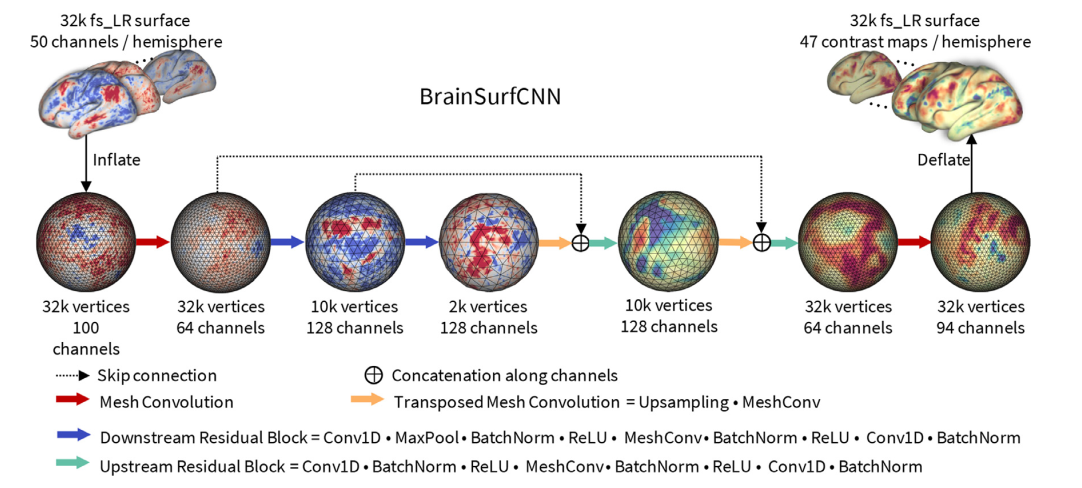
\includegraphics[scale=0.375]{fig/BrainSurfCNN.png}
\caption{{\textcolor{blue}{Fig.2. }{Модель BrainSurfCNN}}}
\label{BrSurf}
\end{figure}

\end{frame}


%----------------------------------------------------------------------------------------------------------


\begin{frame}{Метод (baseline)}
\textbf{Линейная регрессия:}

$$
\boldsymbol{y}_i^k = \boldsymbol{X}_i^k \boldsymbol{\beta}_i^k
$$

$\boldsymbol{y}_i^k$ -- патерн активации ($n_k \times 1$, где $n_k$ -- количество вертексов в $k$-ом парселе в обоих полушариях мозга),

$\boldsymbol{X}_i^k$ -- извлечённые объекты ($n_k \times M$, функциональная матрица связности, где каждый элемент был вычислен как корреляция Пирсона между вертексом и средним временных рядов каждого из $M$ интересующих регионов),

$\boldsymbol{\beta}_i^k$ -- регрессор $k$-го парселя для $i$-го индивида ($M \times 1$). \\[0.2cm]

% Для вычисления модели линейной регрессии была использована 50-компонентная парцелляция, полученная из ICA и предоставленная HCP.

\textbf{Предсказанный патерн активации:}
$$
\qquad\hat{\boldsymbol{y}}_{\text{test}}^k = {\boldsymbol{X}}_{\text{test}}^k \bar{\boldsymbol{\beta}}^k = {\boldsymbol{X}}_{\text{test}}^k \frac{1}{N_{\text{train}}} \sum_{i=1}^{N_{\text{train}}} {\boldsymbol{\beta}}_i^k = \frac{1}{N_{\text{train}}} \sum_{i=1}^{N_{\text{train}}} {\boldsymbol{X}}_{\text{test}}^k {\boldsymbol{\beta}}_i^k
$$

$\bar{\boldsymbol{\beta}}^k$ -- усреднённые веса моделей линейной регрессии для $k$-го парселя, вычисленного по $N_\text{train}$ объектам обучения.   
\end{frame}


%----------------------------------------------------------------------------------------------------------


\begin{frame}{Метрика}
\begin{block}{}

\textbf{\large Dice score}

измеряет степень перекрытия между прогнозируемой контрастностью и целевой картой контрастности для заданного процента $x\%$ наиболее активированных вершин:
    $$
    Dice(x) = \frac{2 | Prediction(x) \cap Target(x)|}{| Prediction(x) | + | Target(x)|},
    $$

\begin{itemize}
    \item $| Prediction(x) |$ -- количество топ-$x\%$ наиболее активированных вершин на прогнозируемой карте контрастности, 
    \item $| Target(x)|$ -- количество топ-$x\%$ наиболее активированных вершин в контрасте,
    \item $| Prediction(x) \cap Target(x)|$ -- количество вершин, которые перекрывают прогнозируемую и целевую карты при заданном пороговом значении.
\end{itemize} 

\end{block}
\end{frame}


%----------------------------------------------------------------------------------------------------------


\begin{frame}{Функция потерь}
\begin{block}{}
%    \footnotesize{The reduction of indexicity in modeling fMRI images of human brain}

{Дан минибатч из $N$ сэмплов: $B=\{\textbf{x}_i\}$.

$\textbf{x}_i$ - целевое многоконтрастное изображение объекта $i$,

$\hat{\textbf{x}}_i$ - соответствующее прогнозируемое изображение контраста,

$d(.)$ -- функция потерь. \\[0.25cm]

\textbf{The reconstructive-contrastive loss (RC loss):}
$$
\mathcal{L}_R = \frac{1}{N} \sum\limits_{i=1}^N d(\hat{\textbf{x}}_i, {\textbf{x}}_i), 
\qquad
\mathcal{L}_C = \frac{1}{(N^2-N)/2} \sum\limits_{\substack{\textbf{x}_j \in B_i, \\ j\neq i}} d(\hat{\textbf{x}}_i, {\textbf{x}}_j),
$$
$$
\mathcal{L}_{RC} = [\mathcal{L}_R - \alpha]_+ + [\mathcal{L}_R - \mathcal{L}_C + \beta]_+.
$$
\\[0.25cm]

$\mathcal{L}_R, \alpha$ -- потери и отступ (margin) для одного и то же объекта (R loss).

$\mathcal{L}_C, \beta$ -- потери и отступ (margin) для разных объектов (C loss). \\[0.2cm]

\textit{Условие:} $(\mathcal{L}_C-\mathcal{L}_R) > \beta$.}
\end{block}

\end{frame}


%----------------------------------------------------------------------------------------------------------


\begin{frame}{Эксперименты}
\begin{figure}
\centering
\includegraphics[scale=0.23]{fig/corr.png}
    \caption{{\textcolor{blue}{Fig.3. }{Нормализованные корреляционные матрицы прогнозируемых и истинных контрастов между испытуемыми для трёх заданий и 39 испытуемых}}}
    \label{BrSurf5}
\end{figure}
\end{frame}


%----------------------------------------------------------------------------------------------------------


\begin{frame}{Эксперименты}
\begin{figure}
\centering
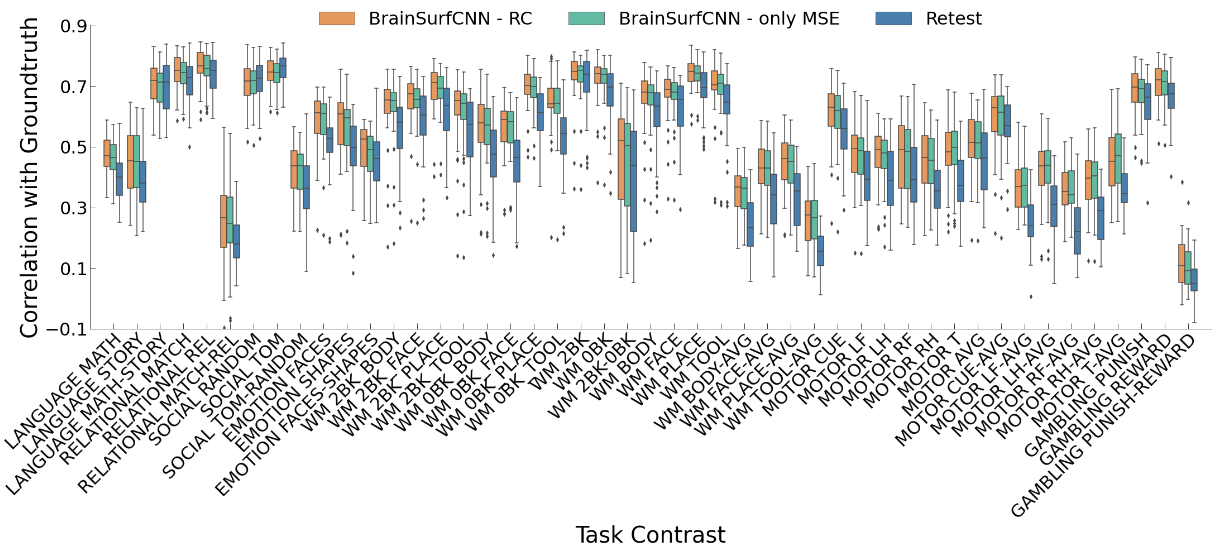
\includegraphics[scale=0.375]{fig/task_contrasts.png}
    \caption{{\textcolor{blue}{Fig.4. } {Корреляция прогнозируемых и истинных контрастов в 47 индивидуальных заданиях}}}
    \label{BrSurf3}
\end{figure}
\end{frame}


%----------------------------------------------------------------------------------------------------------


\begin{frame}{Эксперименты}
\begin{figure}
\centering
\includegraphics[scale=0.33]{fig/fig4.png}
    \caption*{{\textcolor{blue}{Fig.5. } {Визуализация поверхности для сравнения двух заданий у 2 испытуемых. В крайнем правом столбце приведены средние значения контрастов по группе для сравнения}}}
    \label{BrSurf4}
\end{figure}
\end{frame}


%----------------------------------------------------------------------------------------------------------


\begin{frame}{Эксперименты}
\begin{figure}
\centering
\includegraphics[scale=0.33]{fig/fig6.png}
    \caption*{{\textcolor{blue}{Fig.6. } {Точность прогнозов для индивида в 23 надежно прогнозируемых задачах}}}
    \label{BrSurf6}
\end{figure}
\end{frame}


%----------------------------------------------------------------------------------------------------------


\begin{frame}{Список литературы}
\begin{enumerate}
    \footnotesize \item Ngo G. H. et al. 2022. \textcolor{blue}{\href{https://doi.org/10.1016/j.neuroimage.2021.118849}{Predicting individual task contrasts from resting‐state functional connectivity using a surface‐based convolutional network}}. \\

    \item Bernstein-Eliav M., Tavor I. et al. 202. \textcolor{blue}{\href{https://doi.org/10.1177/10738584221130974}{The prediction of brain activity from connectivity: advances and applications}}. \\

    \item Jones O. P. et al. 2017. \textcolor{blue}{\href{https://doi.org/10.1016/j.nicl.2016.12.028}{Resting connectivity predicts task activation in pre-surgical populations}}.\\ 

    \item Tavor I. et al. 201. \textcolor{blue}{\href{https://doi.org/10.1126/science.aad8127}{Task-free MRI predicts individual differences in brain activity during task performance}}.\\

    \item Luckett P. H. et al. \textcolor{blue}{\href{https://doi.org/10.3389/fneur.2022.1055437}{Resting state network mapping in individuals using deep learning}}

    \item Pagani M. et al. \textcolor{blue}{\href{https://doi.org/10.1016/B978-0-323-91688-2.00009-6}{Resting state fMRI connectivity mapping across species: Challenges and opportunities}}

    \item Kumar V. A. et al \textcolor{blue}{\href{https://doi.org/10.1186/s40644-020-00327-w}{The role of resting-state functional MRI for clinical preoperative language mapping}}

    \item Hou X. et al. \textcolor{blue}{\href{https://doi.org/10.1038/s41746-023-00859-y}{Deep-learning-enabled brain hemodynamic mapping using resting-state fMRI}}
    
    \item Rabini G., Ubaldi S., Fairhall S. L. \textcolor{blue}{\href{https://doi.org/10.1038/s42003-023-05400-1}{Task-based activation and resting-state connectivity predict individual differences in semantic capacity for complex semantic knowledge}}

    \item Zheng Y. Q. et al. \textcolor{blue}{\href{https://doi.org/10.1016/j.neuroimage.2022.119418}{Accurate predictions of individual differences in task-evoked brain activity from resting-state fMRI using a sparse ensemble learner}}
    
    \item Duda M. et al. \textcolor{blue}{\href{ https://doi.org/10.1002/hbm.26234}{Reliability and clinical utility of spatially constrained estimates of intrinsic functional networks from very short fMRI scans}}   
    
    \item Duda M., Iraji A., Calhoun V. D. \textcolor{blue}{\href{https://doi.org/10.1109/EMBC48229.2022.9871305}{Spatially constrained ICA enables robust detection of schizophrenia from very short resting-state fMRI}}  

    \item Lin Q. H. et al. \textcolor{blue}{\href{https://doi.org/10.1002/hbm.20919}{Semiblind spatial ICA of fMRI using spatial constraints}}

    \item Wang Z. et al. \textcolor{blue}{\href{https://doi.org/10.1371/journal.pone.0094211}{Temporally and spatially constrained ICA of fMRI data analysis}}
    
    \item Dataset: \textcolor{blue}{\href{https://www.humanconnectome.org/}{Human Connectome Project}} 
\end{enumerate} %\\[0.25cm] 
\end{frame}


%----------------------------------------------------------------------------------------------------------


\begin{frame}{Заключение}
  \begin{itemize}
      \item Были рассмотрены подходы к проблеме исследования функционального картирования мозга
      
      \item Проанализирована литература
      
      \item Намечен план дальнейшего исследования, в частности 2 возможных направления:
      \begin{itemize}
          \item Отображение fMRI в состоянии покоя (Resting state fMRI mapping) 
          \item Пространственно ограниченный ICA fMRI (Spatially constrained ICA fMRI)
      \end{itemize}
      
      \item Были проведены основные эксперименты и посчитаны метрики
      
      \item  Была написана основная часть текста статьи
  \end{itemize} 

\end{frame}

%----------------------------------------------------------------------------------------------------------

\end{document} 